\documentclass[10pt,a4paper]{article}
\usepackage[margin=2.2cm]{geometry}
\usepackage{fontspec}
\usepackage{kotex}
\setmainfont{Apple SD Gothic Neo}
\setsansfont{Apple SD Gothic Neo}
\usepackage{amsmath,amssymb}
\usepackage{graphicx}
\usepackage{booktabs}
\usepackage{caption}
\usepackage[dvipsnames]{xcolor}
\usepackage[colorlinks=true,linkcolor=MidnightBlue,citecolor=MidnightBlue,
            urlcolor=MidnightBlue]{hyperref}
\usepackage{titlesec}
\titleformat{\section}{\large\bfseries}{\thesection}{0.6em}{}
\captionsetup{font=small,labelfont=bf}
\setlength{\parskip}{0.35em}
\setlength{\parindent}{0pt}

\usepackage{mdframed}
\newmdenv[linewidth=0.4pt,linecolor=gray!60,backgroundcolor=gray!5,
          innertopmargin=6pt,innerbottommargin=6pt,skipabove=8pt,skipbelow=8pt]{claimbox}
\newcommand{\claim}[2]{\begin{claimbox}\textbf{주장.} #1\par\smallskip
  \textcolor{gray!70}{\textbf{반증 조건.} #2}\end{claimbox}}

\title{\bfseries 영화는 판에서 가장 큰 임펄스다\\[2pt]
\large $90$일 백필 파일럿 --- 진폭 $4.19$, 그리고 절단은 예상의 세 배}
\author{월드모델 실험실 · 노트 $830$}
\date{2026-08-07}
\begin{document}\maketitle

\section{한 줄}

문패 $6$건 재개의 $0$순위(티처 \#$6$): $813/814/818$ 이 \textbf{가정만} 하고
있던 ``KOBIS $=$ 진폭 큰 안정 도메인'' 전제를 실측했다. $90$일 백필
($2026$-$05$-$04{\sim}08$-$01$ · $90/90$ 성공 · 누적 역행 $0.05\%$): 개봉일 정렬
평균 곡선의 진폭 \textbf{$4.19$} --- 문턱($1.0$)의 $4$배, 내 예측 구간
($1.5{\sim}3.0$)도 위로 뚫었고, \textbf{기존 최대(게임 $1.828$)의 $2.3$배}다.
갈래 $2$: 문패 $3$건의 전제 성립 --- $831$ 합류 사전등록 진행.

\begin{figure}[t]\centering
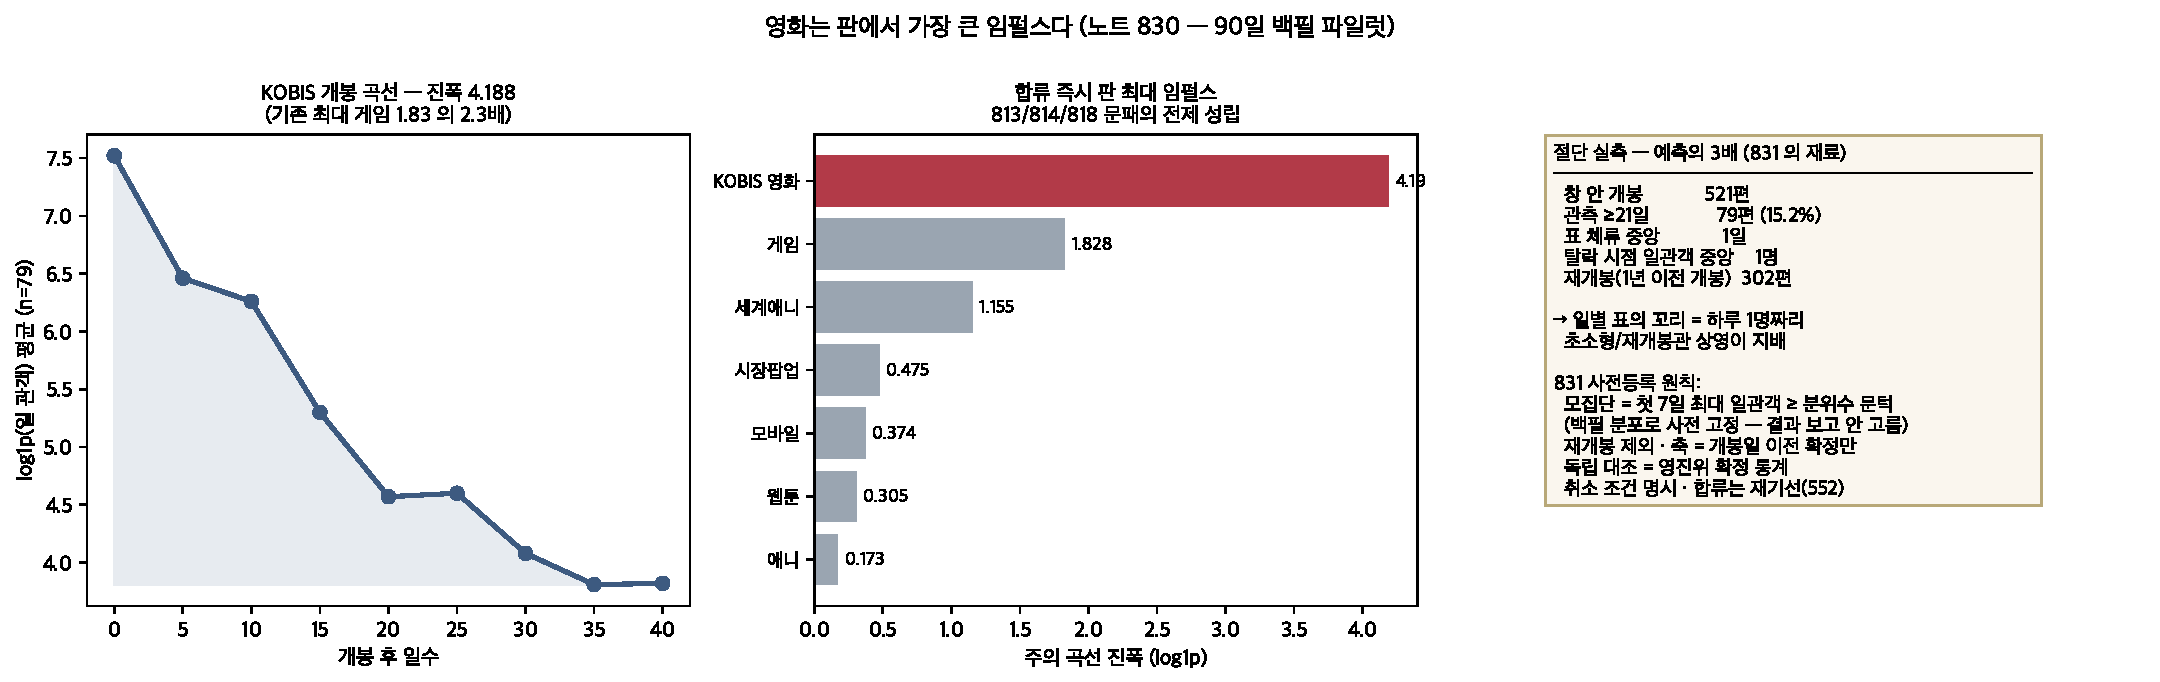
\includegraphics[width=0.99\textwidth]{figs/impulse.pdf}
\caption{왼쪽: 개봉 곡선($n{=}79$). 가운데: 도메인 진폭 순위 --- 영화가 새
$1$위. 오른쪽: 절단 실측과 $831$ 원칙.}
\end{figure}

\section{빗나간 예측이 라벨 정의를 만들었다}

\claim{\textbf{일별 표의 절단은 예상의 $3$배다} --- 창 안 개봉 $521$편 중 관측
$\geq 21$일은 $79$편($15.2\%$ · 내 예측 $50{\sim}80\%$), 표 체류 중앙 $1$일,
탈락 시점 일관객 중앙 \textbf{$1$명}, 재개봉 $302$편. 꼬리는 하루 $1$명짜리
초소형/재개봉관 상영이 지배한다 --- 티처 \#$6$ 이 경고한 생존편향 함정(노트
$658/659$ 계열)의 실물. 따라서 $831$ 의 라벨 모집단은 `전체 표 등장작'이
아니라 \textbf{첫 $7$일 최대 일관객 $\geq$ 분위수 문턱의 상업 개봉작}으로
정의하고(문턱은 이번 백필 분포에서 사전 고정 --- 결과 보고 고르지 않는다),
재개봉 제외 규칙과 독립 대조(영진위 확정 통계)를 취소 조건과 함께 박는다.}
{못 박기도 이번 사이클에 있었다: $829$ 의 ``자기시험 내장''은 문안뿐이었음을
자인 기록하고(\texttt{pairboot.check()} 실제 내장 $+$ 고정물 핀 $+$
CLAIMED\_FIXES $2$행 --- $828$ 이 만든 `문안$\neq$코드' 렌즈에 내가 걸린 사례),
kobis 셀 명명 · 오기($114$편 · 문패 $6$건) 정정. 판 $\rho$ $0.4689$ 그대로 ---
$831$ 합류가 성사되면 \textbf{재기선}(노트 $552$ 관례)이다.}

\end{document}
